% \documentclass{article}
\documentclass[a4paper, 11pt]{report}
% \usepackage{graphicx}
% \usepackage{hyperref}
% \usepackage{algorithm,algorithmic,caption} % lecture 5
% \usepackage{amsmath}
% \usepackage[T1]{fontenc}
% \usepackage{amsfonts}
% \usepackage{enumitem}
% \usepackage{natbib}
% \usepackage{listings}
% \setenumerate[1]{label=\thesection.\arabic*.}
% \usepackage{datetime}
\usepackage[hmargin=2cm, vmargin=2.1cm]{geometry}
\usepackage{../../PW_preamble}
\DeclareMathOperator{\softmax}{softmax}

\renewcommand{\clearpage}{}
\renewcommand{\cleardoublepage}{}

\renewenvironment{abstract}{
\vspace{.5cm}
\begin{center}
\textbf{Abstract} \\
\vspace{.1cm}
}{\end{center}}

\setlength{\parindent}{0pt}

% \setlength{\parskip}{0.5\baselineskip}%
% \setlength\parindent{0pt}

\begin{document}

\doctype{Practical Work}
\coursetitle{Graphs in Machine Learning}
\semester{MVA Fall 2019}
\instructor{Michal Valko}
\teachingassistant{Omar Darwiche-Domingues, Pierre Perrault}
\student{Antoine Moulin}
\worknumber{3}
\workdate{December 6}

% 	\title{TP3: Graph Neural Networks}
% 	\author{omar (dot) darwiche-domingues (at) inria.fr \\
% 			pierre (dot) perrault (at) inria.fr}
% 	\date{December 6, 2019}
\maketitle

\begin{abstract}
	The report and the code are due in 2 weeks (deadline 23:59, 20/12/2019). You will find instructions on how to submit the report on piazza, as well as the policies for scoring and late submissions.
\end{abstract}

\chapter{Neural Relational Inference}

This practical session is based on the paper \href{https://arxiv.org/pdf/1802.04687.pdf}{\emph{Neural Relational Inference for Interacting Systems}} by Kipf et al., 2018.

We will use the following material provided by Marc Lelarge and Timoth\'ee Lacroix: \url{https://github.com/timlacroix/nri_practical_session}. 

\section{Motivation and problem formulation}
A wide range of dynamical systems can be seen as a group of interacting components. For example, we can think of a set of 2-dimensional particles coupled by springs. Assume that we are given only a set of trajectories of such interacting dynamical system. How can we learn its dynamical model in an unsupervised way?

Formally, we are given as input a set of trajectories of $N$ objects, and each trajectory has length $T$. Each object $i$, for $i=1,\ldots, N$, is represented by a vertex $v_i$. Let $\mathbf{x}_i^t$ be the feature vector of object $i$ at time $t$ (e.g., position and velocity) with dimension $D$. Let $\mathbf{x}^t = \{\mathbf{x}_1^t, \ldots, \mathbf{x}_N^t\}$ be the set of features of all $N$ objects at time $t$ and let $\mathbf{x}_i = (\mathbf{x}_i^1, \ldots, \mathbf{x}_i^T)$ be the trajectory of object $i$. The input data can be stored in a 3-dimensional array $\mathbf{x}$ of shape $N\times T \times D$, denoted by $\mathbf{x} = (\mathbf{x}^1, \ldots, \mathbf{x}^T)$, such that $\mathbf{x}_{i,t,d}$ is the $d$-th component of the feature vector of object $i$ at time $t$. 

In addition,  we assume that the dynamics can be modeled by a graph neural network (GNN) given an unknown graph $\mathbf{z}$ where $\mathbf{z}_{i,j}$ represents the discrete edge type between objects $v_i$ and $v_j$.

In this context, we want to learn, simultaneously:

\begin{itemize}
	\item The edge types $\mathbf{z}_{i,j}$ (\textbf{edge type estimation}); 
	\item A model that, for any time $t$, takes $\mathbf{x}^t$ as input and predicts $\mathbf{x}^{t+1}$ as output (\textbf{future state prediction}).
\end{itemize}

\section{Model}

The Neural Relational Inference (NRI) model consists of:

\begin{itemize}
	\item An \textbf{encoder} that uses trajectories $\mathbf{x} = (\mathbf{x}^1, \ldots, \mathbf{x}^T)$ to infer pairwise interaction vectors $\mathbf{z}_{i, j} \in \mathbb{R}^K$ for $i, j$ in $\{1, \ldots, N \}$, where $K$ is the number of \emph{edge types}.
	\item A \textbf{decoder} that takes $\mathbf{x}^t$ and $\mathbf{z} = \{\mathbf{z}_{i, j}\}_{i,j}$ as input to infer $\mathbf{x}^{t+1}$.
\end{itemize}

Both the encoder and the decoder are implemented using graph neural networks. For more details, read Section 3 of the paper \href{https://arxiv.org/pdf/1802.04687.pdf}{here}. \\


\chapter{Questions}

Complete the code in the following notebook

\url{https://github.com/timlacroix/nri_practical_session/blob/master/NRI_student.ipynb}

and answer the questions below in your report. \textbf{For the report, no code submission is required}. Note that this Github repository contains a \texttt{solutions} folder, which you are allowed to use to complete the notebook. 

\begin{enumerate}
	\item \textbf{Explain what are the edge types $\mathbf{z}_{i,j}$.}
	
	The edge types correspond to different kinds of interactions between the components of a system represented as nodes. For instance, in the case of the mass-spring system studied here, there are two edge types: one for the presence of a spring between two masses and one for the absence.
	
	\item \textbf{In the NRI model, explain how the encoder and the decoder work.}
	
	\begin{itemize}
	    \item \textbf{Encoder}. The goal of the encoder is to infer interactions $\mathbf{z}$ given the trajectories $\mathbf{x}$. More precisely, it consists of a GNN trained on the fully-connected graph formed by the atoms and their pairwise interactions. It learns an embedding of the nodes and apply two passes before returning a distribution $q_{\phi} \left( \mathbf{z} | \mathbf{x} \right)$ that is then used for sampling the edge types (after a relaxation using Gumbel distribution). The passes (node to edge and edge to node) are done as followed (equations from the paper ; $f_{emb}, f_{e}^{1}, f_{v}^{1}, f_{e}^{2}$ are MLPs):
	    
	    \begin{equation*}
	        \begin{aligned}
	        \mathbf{h}_{j}^{1} &= f_{emb} \left( \mathbf{x}_{j} \right) \\
	        \mathbf{h}_{(i, j)}^{1} &= f_{e}^{1} \left( \left[ \mathbf{h}_{i}^{1}, \mathbf{h}_{j}^{1} \right] \right) & (v \rightarrow e) \\
	        \mathbf{h}_{j}^{2} &= f_{v}^{1} \left( \sum_{i \neq j} \mathbf{h}_{(i, j)}^{1} \right) & (e \rightarrow v) \\
	        \mathbf{h}_{(i, j)}^{2} &= f_{e}^{2} \left( \left[ \mathbf{h}_{i}^{2}, \mathbf{h}_{j}^{2} \right] \right) & (v \rightarrow e) \\
	        q_{\phi} \left( \mathbf{z}_{ij} | \mathbf{x} \right) &= \softmax \left( \mathbf{h}_{(i, j)}^{2} \right)
	        \end{aligned}
	    \end{equation*}
	    
	    An important thing to notice here is that the edge embeddings are not just used to pass messages between the nodes but they are used for edge classification as well.
	    
	    \item \textbf{Decoder}. The goal of the decoder is to predict future continuation of the dynamics by modeling $p_{\theta} \left( \mathbf{x}^{t+1} | \mathbf{x}^{t}, \dots, \mathbf{x}^{1}, \mathbf{z} \right)$. Once the interaction graph $\mathbf{z}$ is learned, the decoder uses multiple GNNs in parallel (one for each edge type) and try to predict multiple time steps instead of just one (in order to avoid degenerate decoders). Depending on the assumptions (e.g. Markov assumption), one can model the decoder as in the section 3.4 from the paper, or use a recurrent decoder as in the section 3.5.
	\end{itemize}
	
	\item \textbf{Explain the LSTM baseline used for joint trajectory prediction. Why is it important to have a "burn-in" phase?}
	
	The LSTM baseline is formed by (i) an encoder that learns an embedding for each node, (ii) a LSTM that is trained on the joint embeddings (i.e the input is the concatenation of all the embeddings and the input size is the number of atoms multiplied by the size of the embedding) and (iii) a decoder that maps the output of the LSTM to the original space and that corresponds to the prediction of future steps of the trajectories. Unlike the "single" LSTM baseline that uses one LSTM for each atom and shared weights for all the LSTMs, training only one LSTM on the joint embeddings allows having more weights to catch the dynamics of the system.
	
	It is important to have a "burn-in" phase to make a fair comparison with the NRI model. Indeed, unlike the LSTM baseline, the NRI model trains on whole trajectories. Hence, to make sure the LSTM also has access to the the first part of the trajectory, the real inputs are given during the "burn-in" phase.
	
	\item \textbf{Show and explain the difference between the negative log-likelihood before and after the burn-in phase.}
	
	In figure \ref{fig:q4-nll} are shown the negative log-likelihoods when predicting 10 and 5 steps, respectively.
	
	\begin{figure}[!h]
	    \centering
	    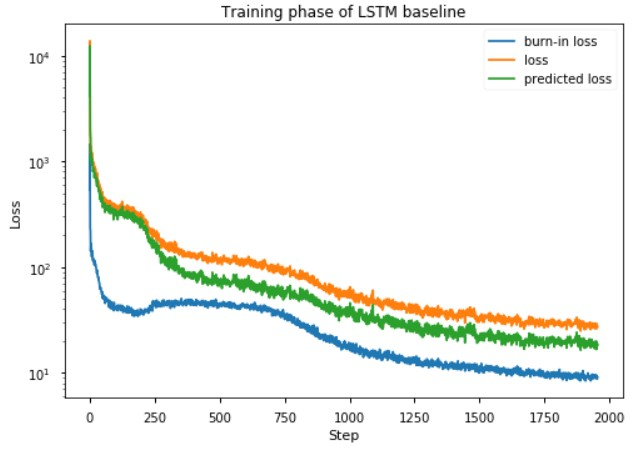
\includegraphics[width=.49\textwidth]{images/q4_10steps.jpg}
	    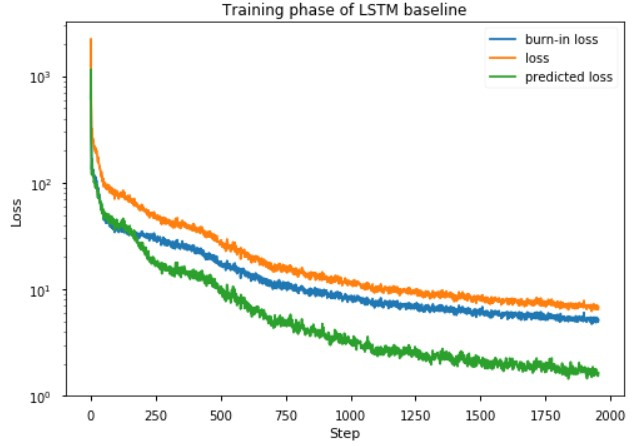
\includegraphics[width=.496\textwidth]{images/q4_5steps.jpg}
	    \caption{Evolution of the negative log-likelihood for each phase (and the total loss) during the training. On the left, 10 steps are predicted successively. On the right, 5 steps are predicted.}
	    \label{fig:q4-nll}
	\end{figure}
	
	When predicting 10 steps, we see that after the burn-in phase, the negative log-likelihood is always higher than before the burn-in phase. When predicting 5 steps, it is the opposite. These differences could be explained by the fact that after the burn-in phase, the LSTM is enough trained to well predict future steps and that is why predicting only 5 steps lead to a lower loss after the burn-in phase. But when we are trying to predict 10 steps in a row, it seems a bit large and the error accumulates too much, leading to a much higher prediction loss than before.
	
	\item \textbf{Consider the problem of trajectory prediction. What are the advantages of the NRI model with respect to the LSTM baseline?}
	
	An advantage of the NRI model with respect to the LSTM baseline is that is uses different neural networks for different edge types. It explicitly specifies that the behavior should be different depending on the edge type. Besides, because it is trained to predict multiple time steps, it is better than the LSTM to make long term predictions.
	
	\item \textbf{Consider the training the of NRI model. What do you notice about the edge accuracy during training? Why is this surprising?}
	
	In figure \ref{fig:q6-edge-acc}, it seems that the edge accuracy increases quickly during the training: in one epoch, it reached 0.9. It may look surprising because on the other hand, we can see in the table 1 of the article that the LSTM baselines do not even reach $0.6$. But except that, the edge accuracy does not look so surprising.
	
	\pagebreak
	
	\begin{figure}
	    \centering
	    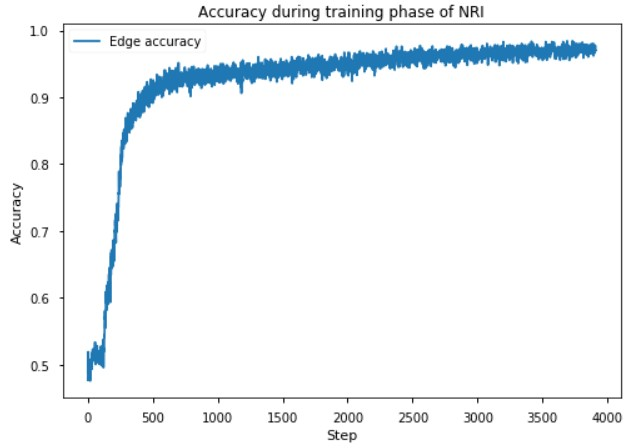
\includegraphics[scale=.8]{images/q6_edge_acc.jpg}
	    \caption{Edge accuracy during the training of NRI model.}
	    \label{fig:q6-edge-acc}
	\end{figure}
	
	\item \textbf{What do you expect to happen with the NRI model when there is no interaction between the objects?}
	
	When there is no interaction between the objects, we could expect the NRI model to fail. Indeed, if the objects are independent, the bias induced by the graph structure (which supposes that, somehow, the objects are in relation) could possibly create mistakes.
	
\end{enumerate}

\end{document}